\documentclass{article}

% Language setting
% Replace `english' with e.g. `spanish' to change the document language
\usepackage{biblatex} %Imports biblatex package
\addbibresource{../Lab2/refs.bib}
\usepackage{enumitem}
\usepackage[english]{babel}
\usepackage{array}
\usepackage{amsmath}
\usepackage{pythonhighlight}
\usepackage{multirow}
\newcolumntype{P}[1]{>{\centering\arraybackslash}p{#1}}
\newcolumntype{M}[1]{>{\centering\arraybackslash}m{#1}}

% Set page size and margins
% Replace `letterpaper' with `a4paper' for UK/EU standard size
\usepackage[letterpaper,top=2cm,bottom=2cm,left=3cm,right=3cm,marginparwidth=1.75cm]{geometry}

\usepackage{amsmath}
\usepackage{graphicx}
\usepackage[colorlinks=true, allcolors=blue]{hyperref}
\usepackage{setspace}
\usepackage{booktabs}
\usepackage[T1]{fontenc}
\usepackage{longtable}
\doublespacing

\begin{document}
\newcommand{\Fig}[3]{\begin{figure}[!h!]\centering\includegraphics[width=0.5\linewidth]{#1}\caption{#2}\label{#3}\end{figure}}
\begin{titlepage}

\centering
\scshape
\vspace{\baselineskip}

%
\rule{\textwidth}{1.6pt}\vspace*{-\baselineskip}\vspace*{2pt}
\rule{\textwidth}{0.4pt}

{\Huge \textbf{\textsc{ Cold Work and Annealing \\
\vspace{15pt}}}}

\rule{\textwidth}{0.4pt}\vspace*{-\baselineskip}\vspace{3.2pt}
\rule{\textwidth}{1.6pt}\vspace{6pt}
\centerline{\textit{University of Illinois at Urbana-Champaign}} 
\centerline{\textit{Department of Nuclear, Plasma, and Radiological Engineering}}
\vspace{1.5\baselineskip}


\large \centerline{\textbf{Author:} Nathan Glaser}
\large \centerline{\textbf{Net-ID:} nglaser3}
\quad

\vfill
\large \centerline{October 2, 2024}
%
\pagenumbering{gobble}
\end{titlepage}

\tableofcontents
\newpage
\pagenumbering{arabic}
 
\section{Abstract}

Prior to implementation of a material in an engineering setting, there is a prerequisite amount of knowledge of the material properties. A useful mechanism to determine material properties is the utilization of phase diagrams. From phase diagrams, we can determine the quantity of some phase micro-structure within the material mixture. In conjunction with prior knowledge of the various material properties of the phases within the phase diagram, much meaningful information can be gleaned. Further, often whenever an investigation of a material includes reading a phase diagram, casting is involved in the formation of the material. Thus, the effect of casting on the macro-structure formations in the mixture is extremely important to have a grasp of. To investigate the aforementioned topics, we investigated the cooling curve of the Bi-Sn system, and investigated the macro-structures of various Aluminum mixtures dependant on material composition, casting temperature, and casting mold type. We determined the cooling curve of various compositions of the Bi-Sn system and, from these curves, extracted the liquidus, solidus, and solvus points, when applicable. We found our experimentally determine inflection points to be a near fit to the theoretical phase-diagram found from \cite{nist}. Further, we determined that sand cast mold specimens cooled much slower, and more uniformly, causing a hole to form at the center of the specimen; whereas graphite cast mold specimens had a divot form at the top ---- where the air was the main coolant ---- as the top cooled much slower than the sides and bottom. Further, we determined that Titanium had the most impact per weight-percent added to the system on the system's grain structure. Finally, we determined that a decrease in super-heat and a presence of specimen agitation during cooling led to more columnar and large granules. 


\newpage
\section{Introduction}
\subsection{Phases and Components}
To begin, single-element materials can have different grain-structures depending on the mechanism utilized in cooling. Further, material mixtures can have different grain structures per element at some given temperature. The grain-structure is called a phase, and the individual phases and elements within a mixture are called components. 


\subsection{Phase Diagrams}
Phase Diagrams present the composition of a mixture as function of temperature and weight-percent of the components. A sample Phase Diagram is shown below in Fig. \ref{fig:gen_phasediag}.

\begin{figure}[!h!]
    \centering
    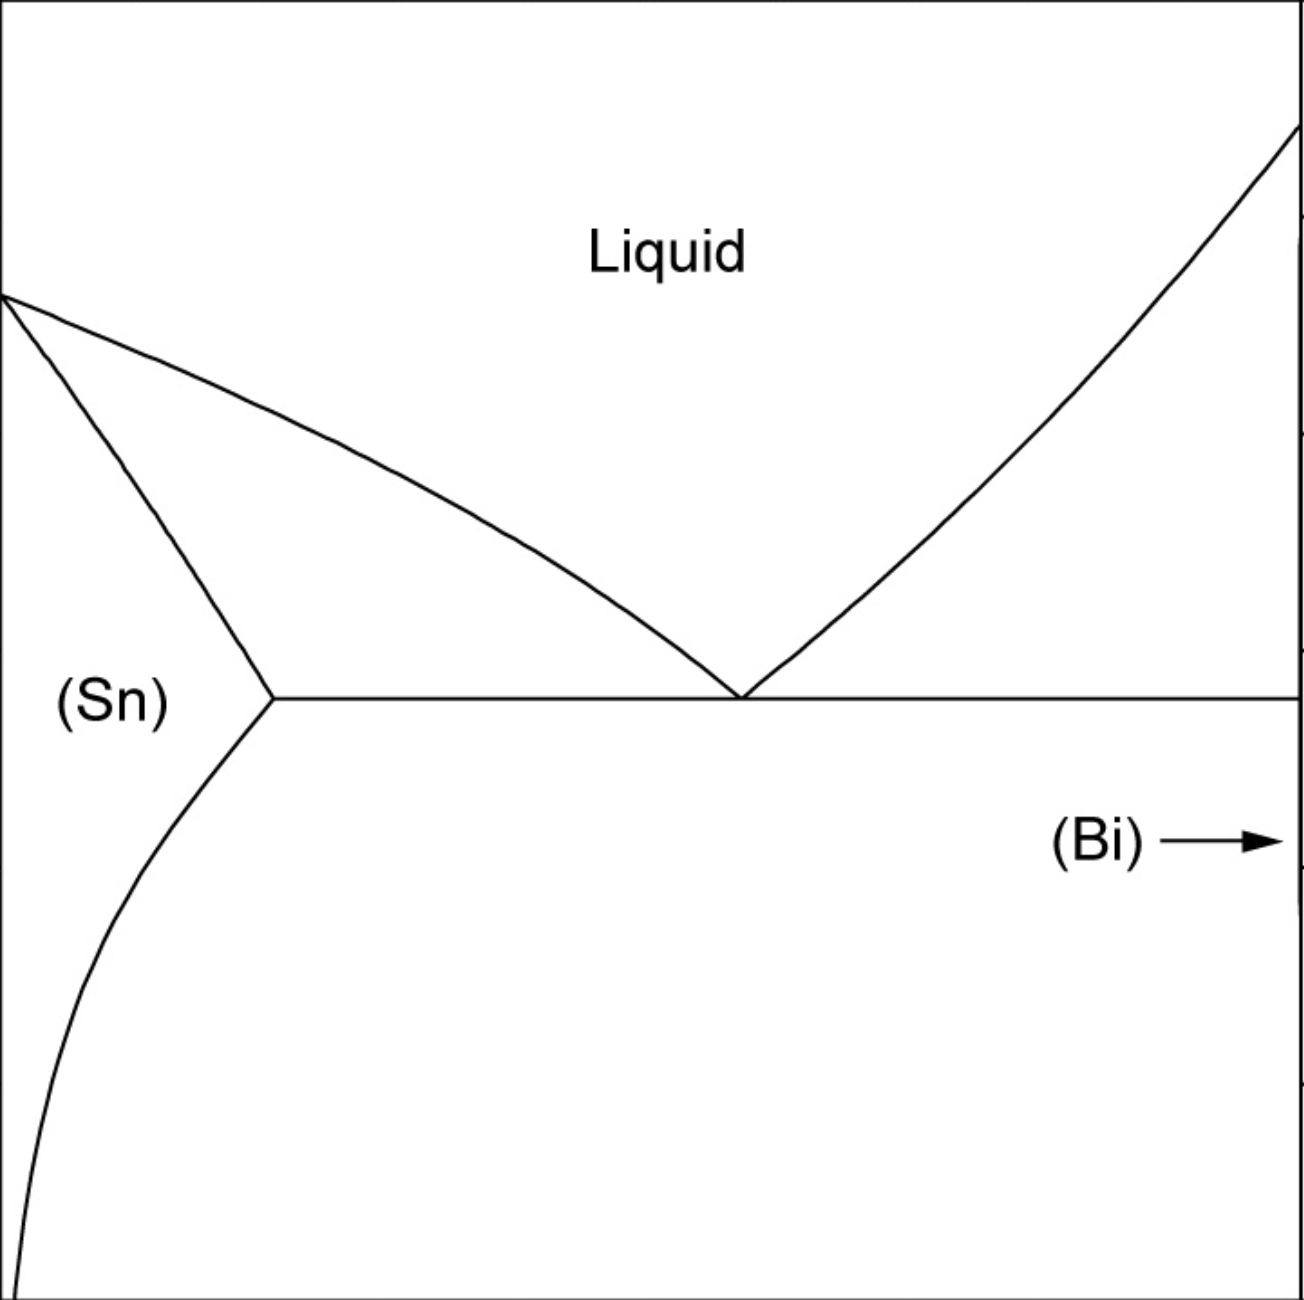
\includegraphics[width=0.5\linewidth]{Lab4/bisn_phasediagram.png}
    \caption{Phase Diagram of Bi-Sn system}
    \label{fig:gen_phasediag}
\end{figure}

Utilizing this figure, we will learn the basics of phase diagrams. The top most region is where the entire system is liquid. left section immediately below Liquid is where the system will be liquid with some solids of Sn forming, conversely for the right section immediately below the liquid. Further, the left most section labeled with $(Sn)$ is $\alpha$-phase Sn. The micro structure of the Sn in this region will appear different than that in the bottom center region. The liquidus point is the top most line in which solids begin forming, the solidus is the line in which everything below is a pure solid. Finally, the point in which the liquidus and solidus meet, where the right mixed and left mixed region meet, is denoted as the eutectic point.


\newpage
\section{Theoretical Models}
We did not employ any theoretical models in our data-processing. 

\section{Experimental Methods}

All experimental methods outlined in this sections were conducted so as to mirror the procedure undertaken in \cite{manual}. We did not form our own compositions, nor place the compositions into crucibles or into the furnace itself. We simply removed pre-made samples from the furnaces. The procedures we undertook are detailed in the following list:

\begin{itemize}
    \item[1.] We removed the 5\% and 100\% weight-percent Bismuth Bi-Sn specimen from the furnaces, maintained at 350 $^o$C. 
    \item[2.] After removal from the furnace, we immediately placed a thermocouple in the specimens, and began collecting the cooling curve of each specimen. We collected data for approximately 10 minutes.
    \item[3.] Finally, to determine the points of inflection we simply found the places in the curve in which the slope drastically changed, and then recorded these in the lab computer. 
\end{itemize}


\newpage
\section{Results}
To begin, we plotted the cooling curve for pure Tin and 90\% Bismuth by weight fraction. The liquidus is marked with a black dotted line, on the temporal axis for clarity, and the solidus for the latter figure is marked with a maroon dotted line, again on the temporal axis for clarity. The true liquidus and solidus points are the intercepts between the curve and their respective dotted lines. 

\begin{figure}[!h!]
    \centering
    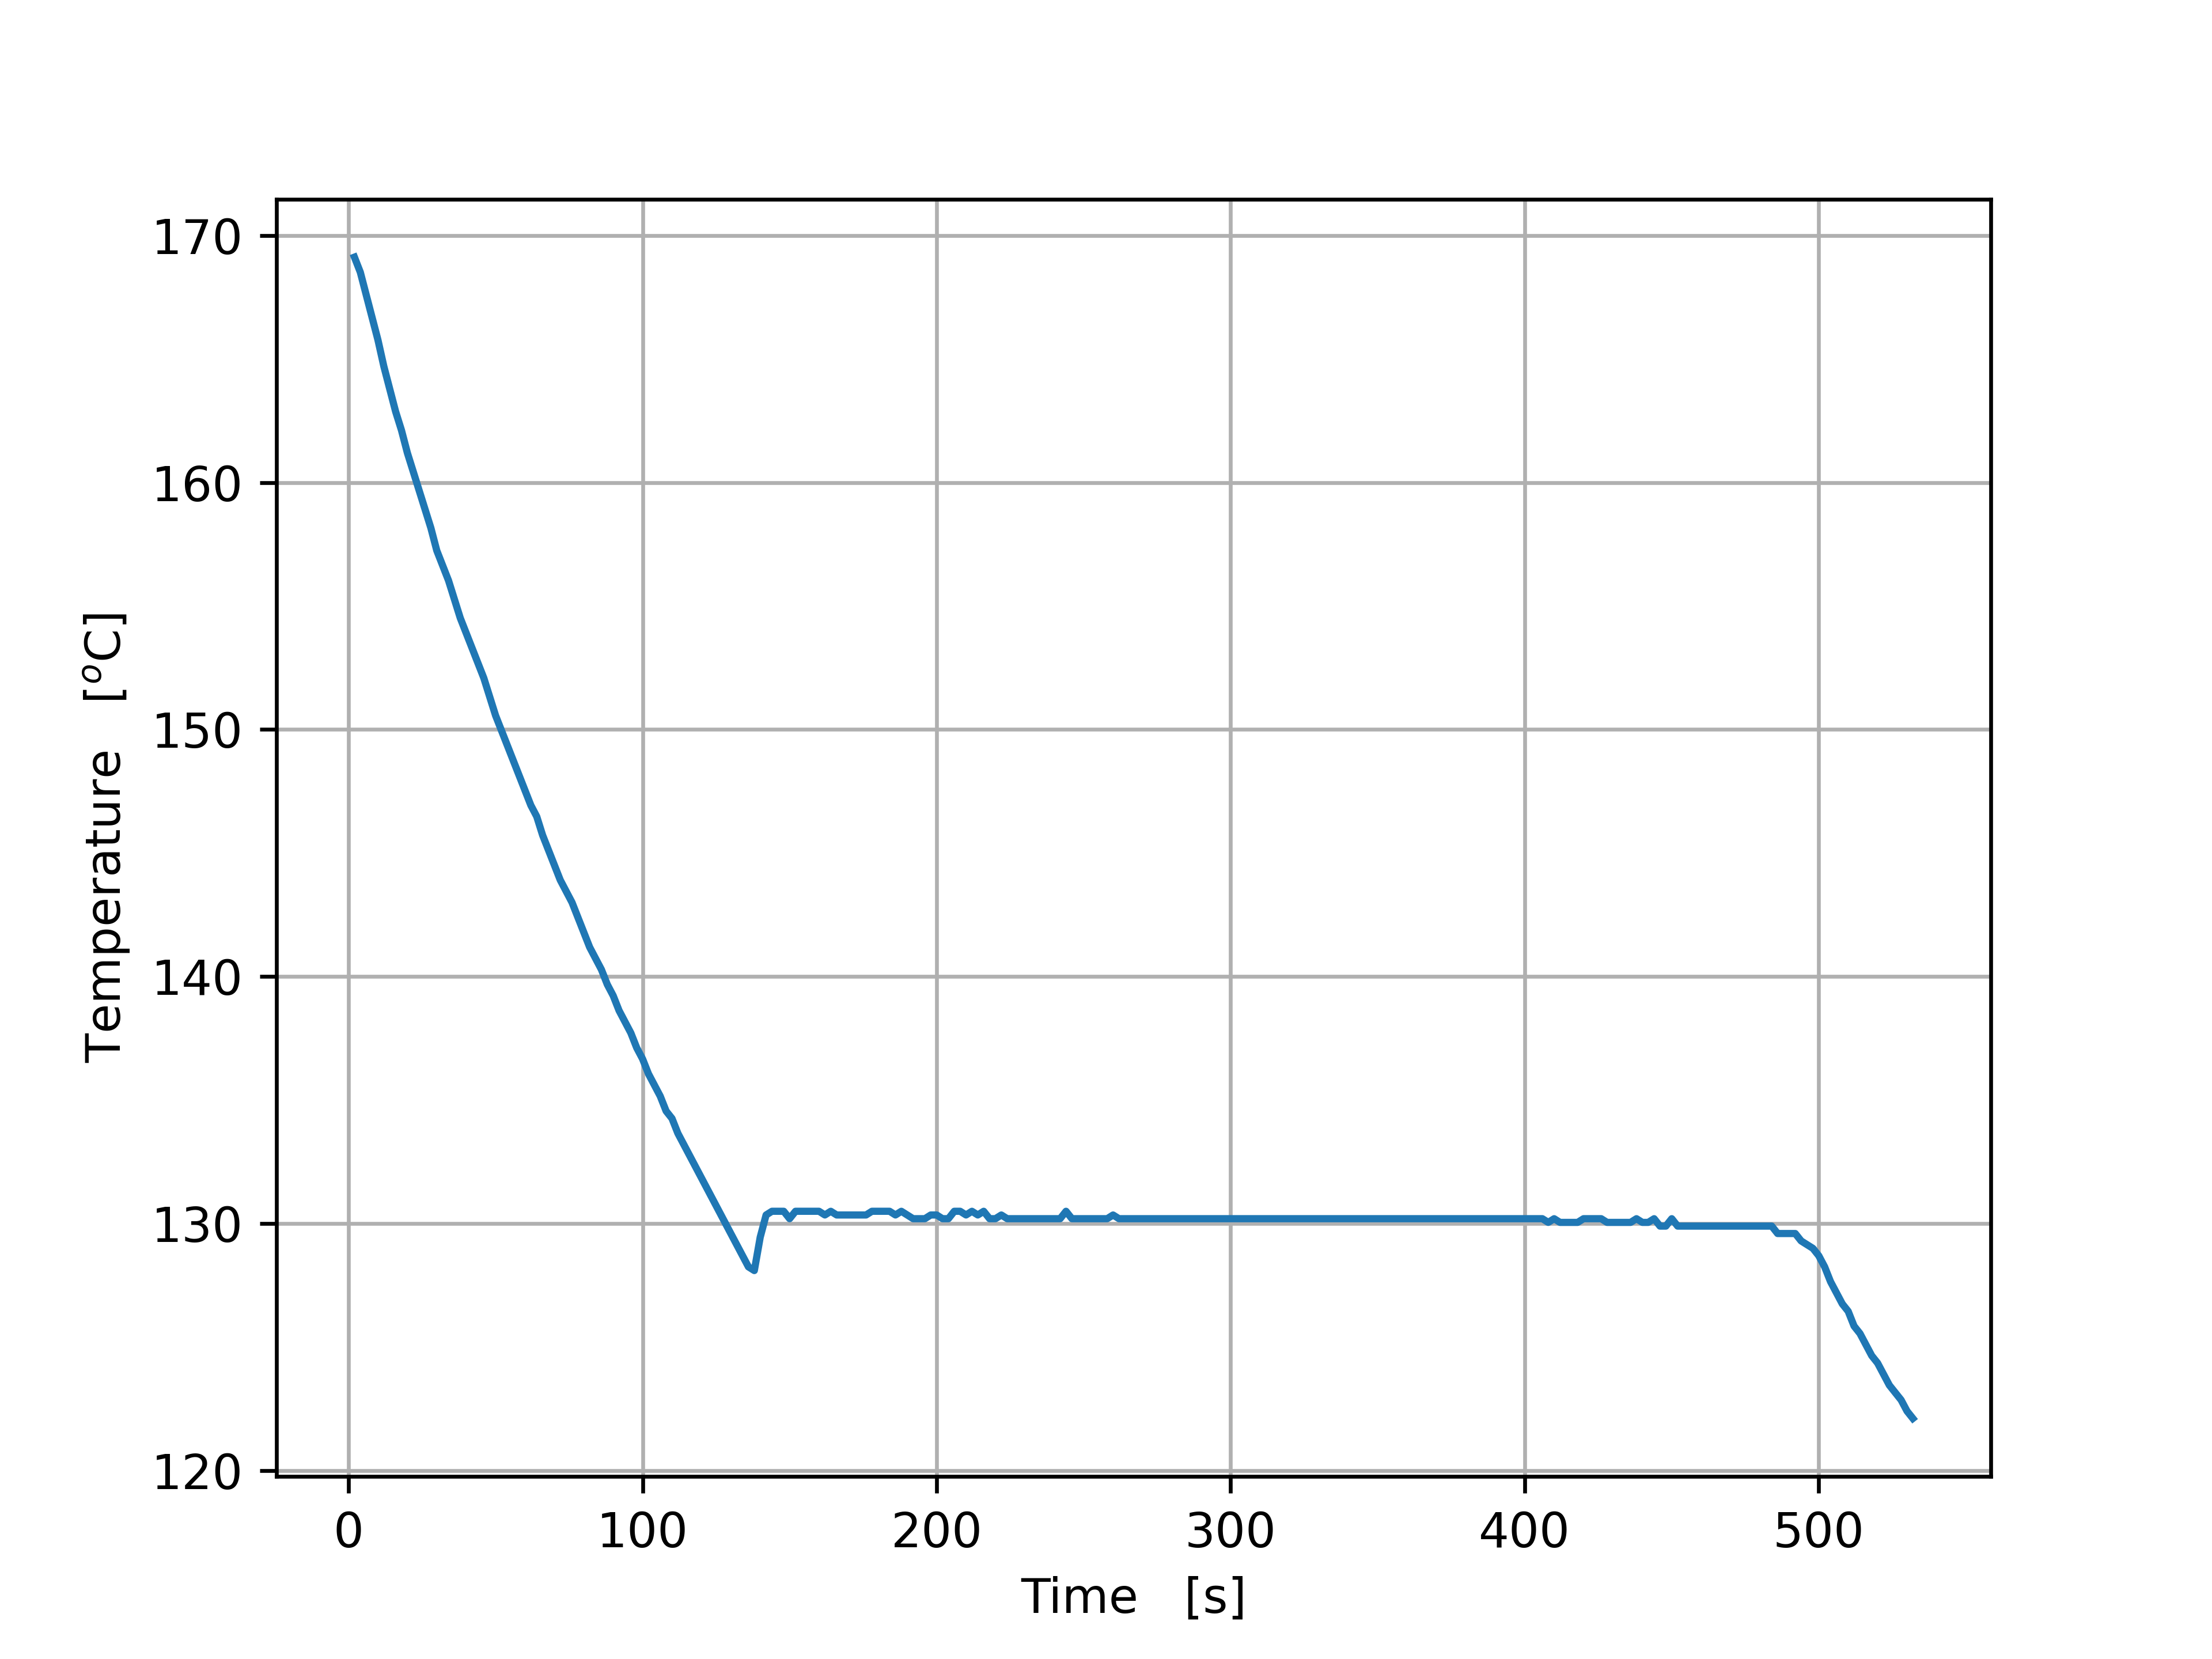
\includegraphics[width=0.5\linewidth]{plots/q1_00.png}
    \caption{Cooling Curve of Pure Tin}
    \label{fig:q1-00}
\end{figure}

\begin{figure}[!h!]
    \centering
    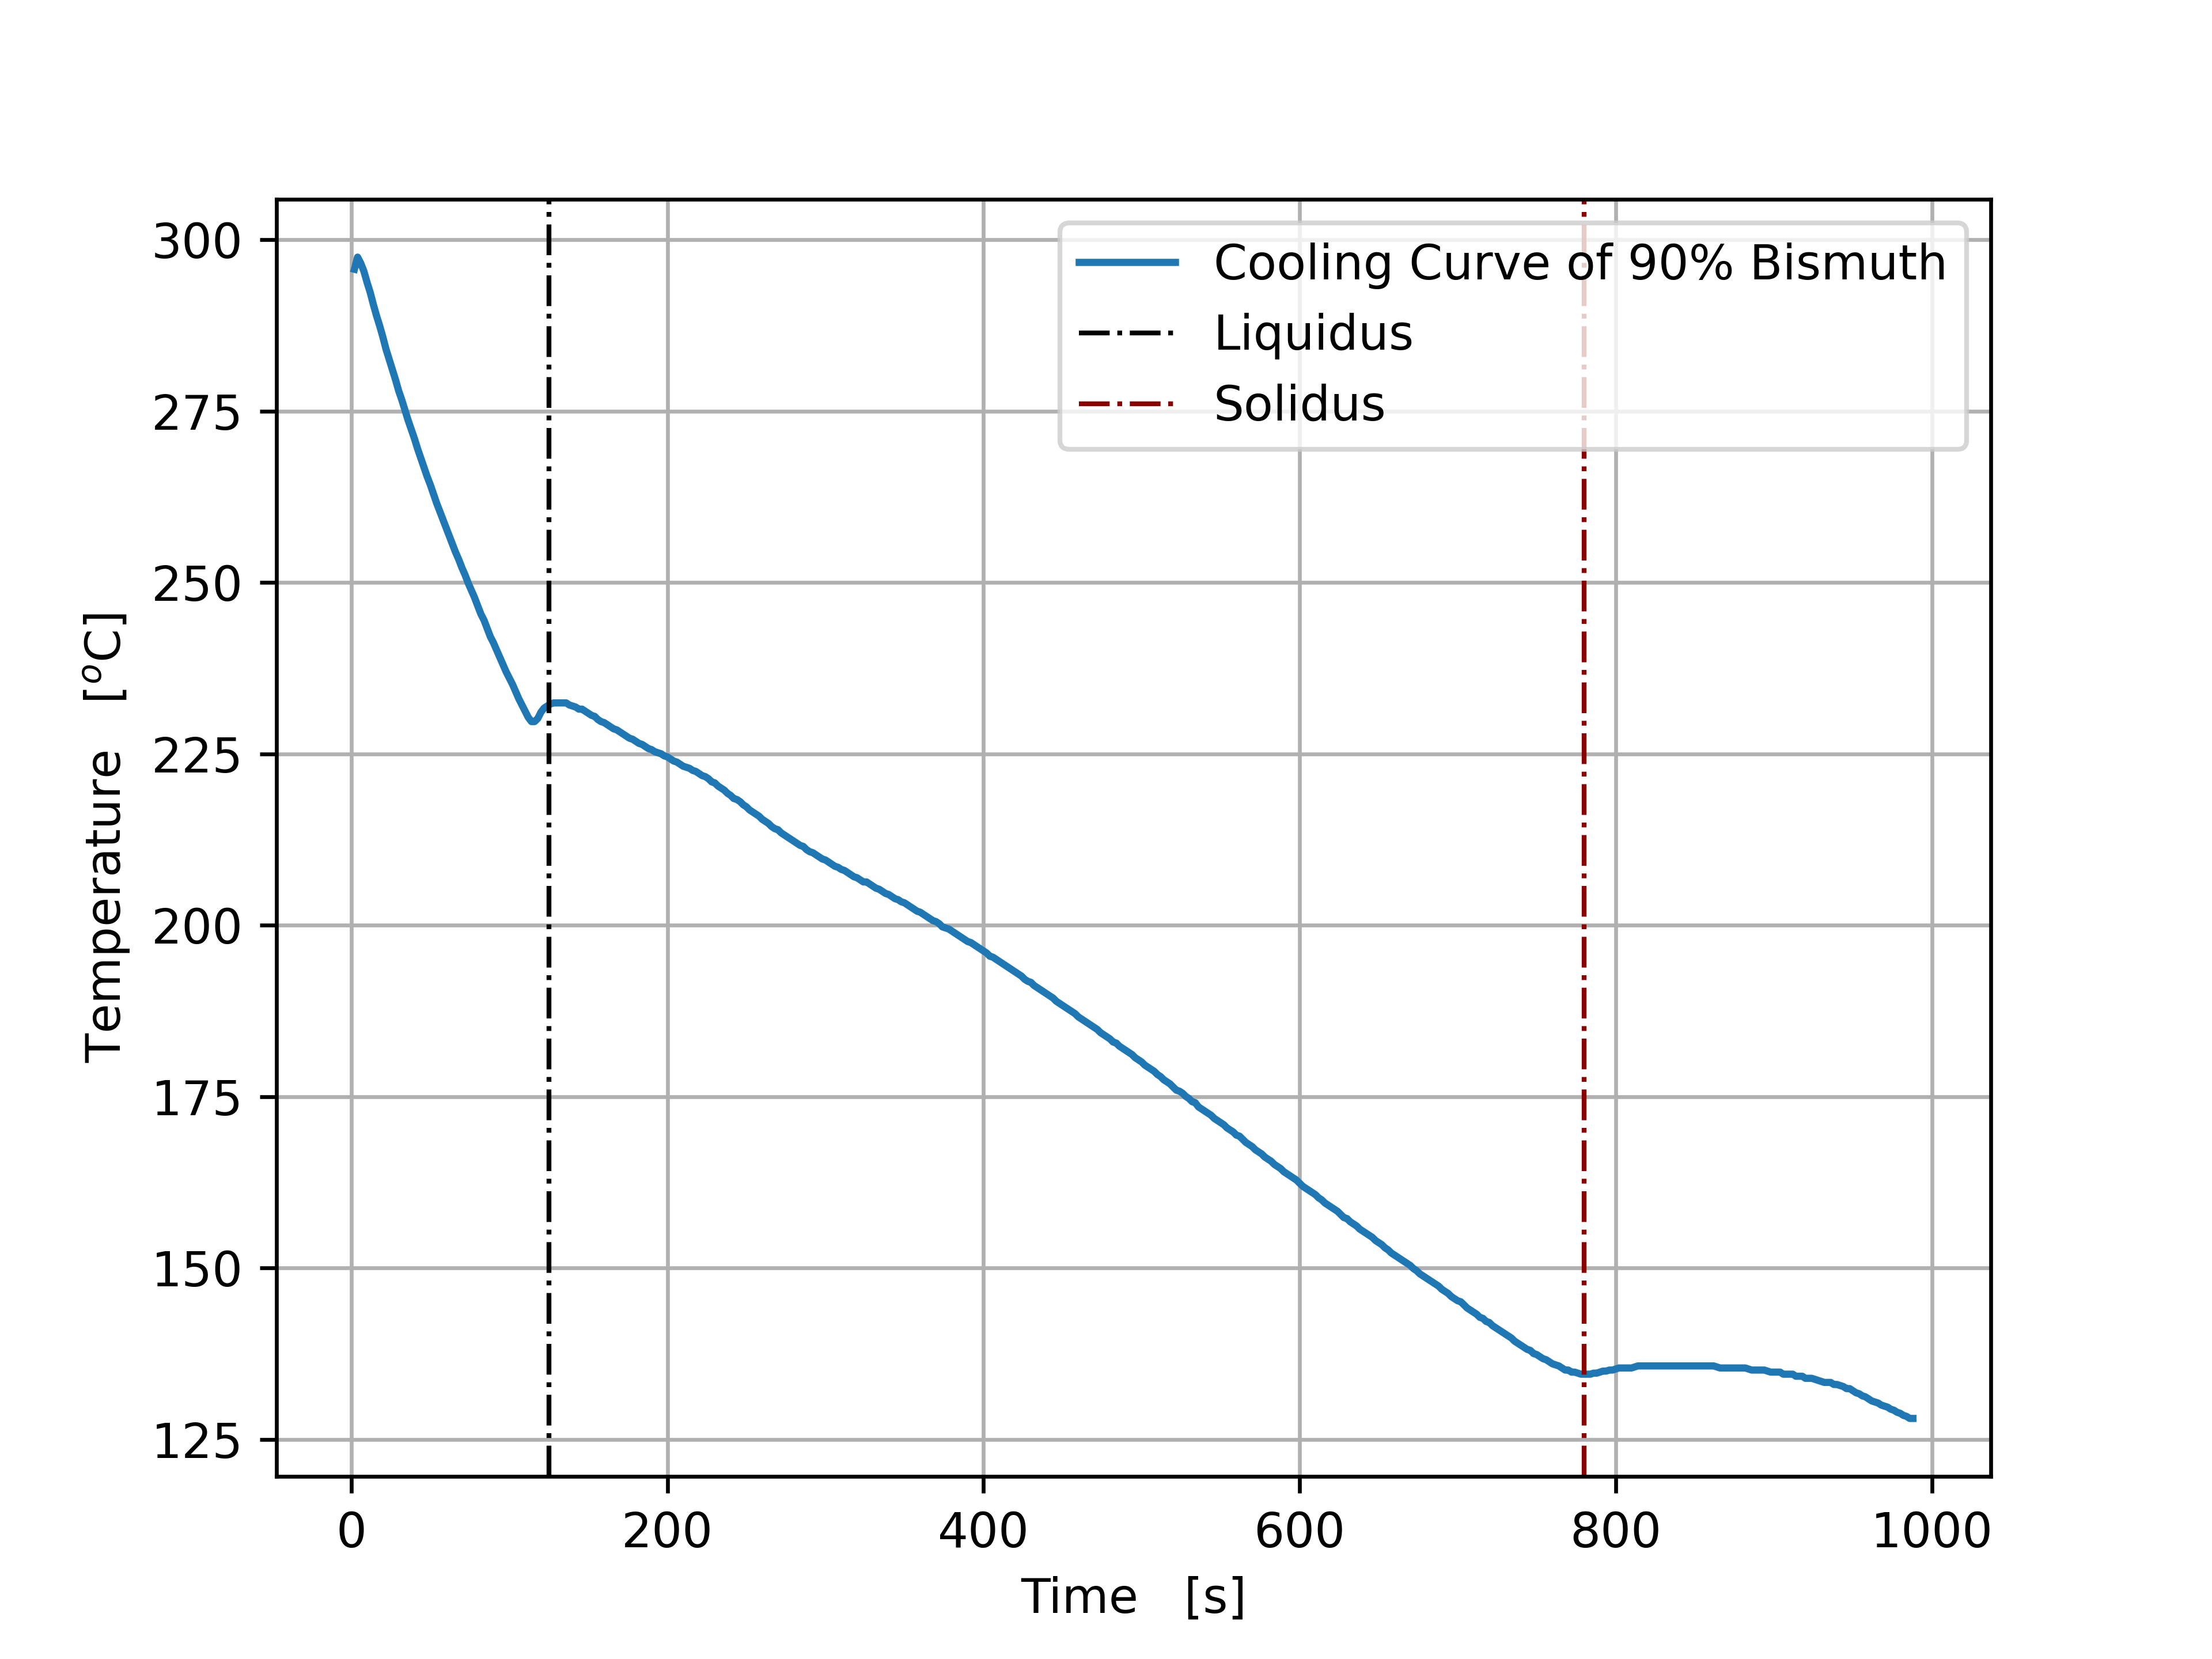
\includegraphics[width=0.5\linewidth]{plots/q1_90.png}
    \caption{Cooling Curve of 90\% Weight-Fraction Bismuth}
    \label{fig:q1-90}
\end{figure}

To continue, We plotted the cooling curves of pure tin, 25\% weight-fraction bismuth, 50\% weight-fraction bismuth, and 55\% weight-fraction bismuth. Alongside, we identified the micro-structure of each mixture. These are presented along-side each other for clarity. 

\newpage

\begin{figure}[!h!]
    \centering
    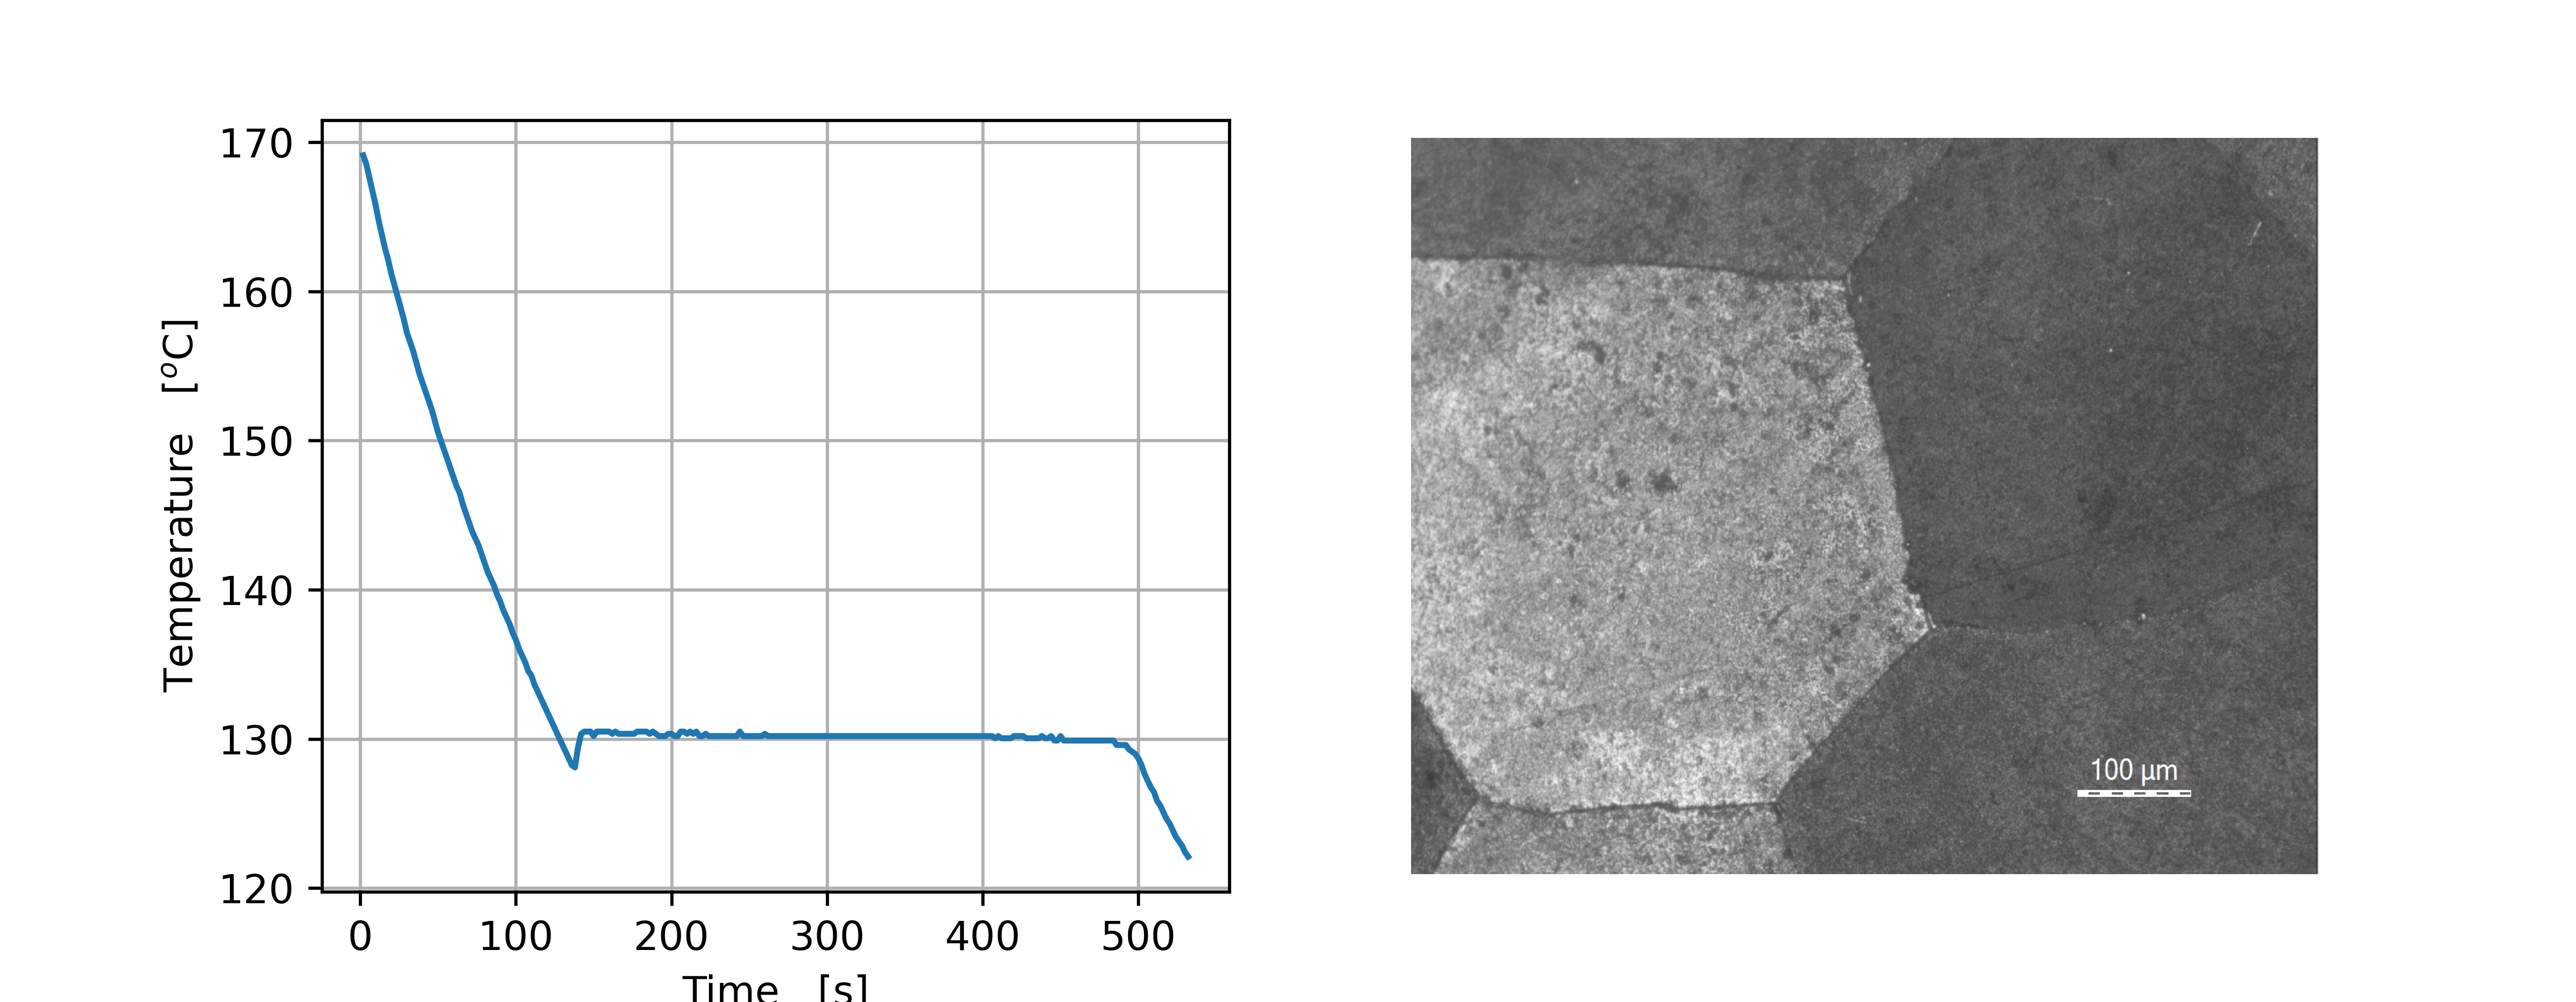
\includegraphics[width=1\linewidth]{plots/q2_00.png}
    \caption{Pure Tin cooling curve and micro-structure}
    \label{fig:q2-00}
\end{figure}

\begin{figure}[!h!]
    \centering
    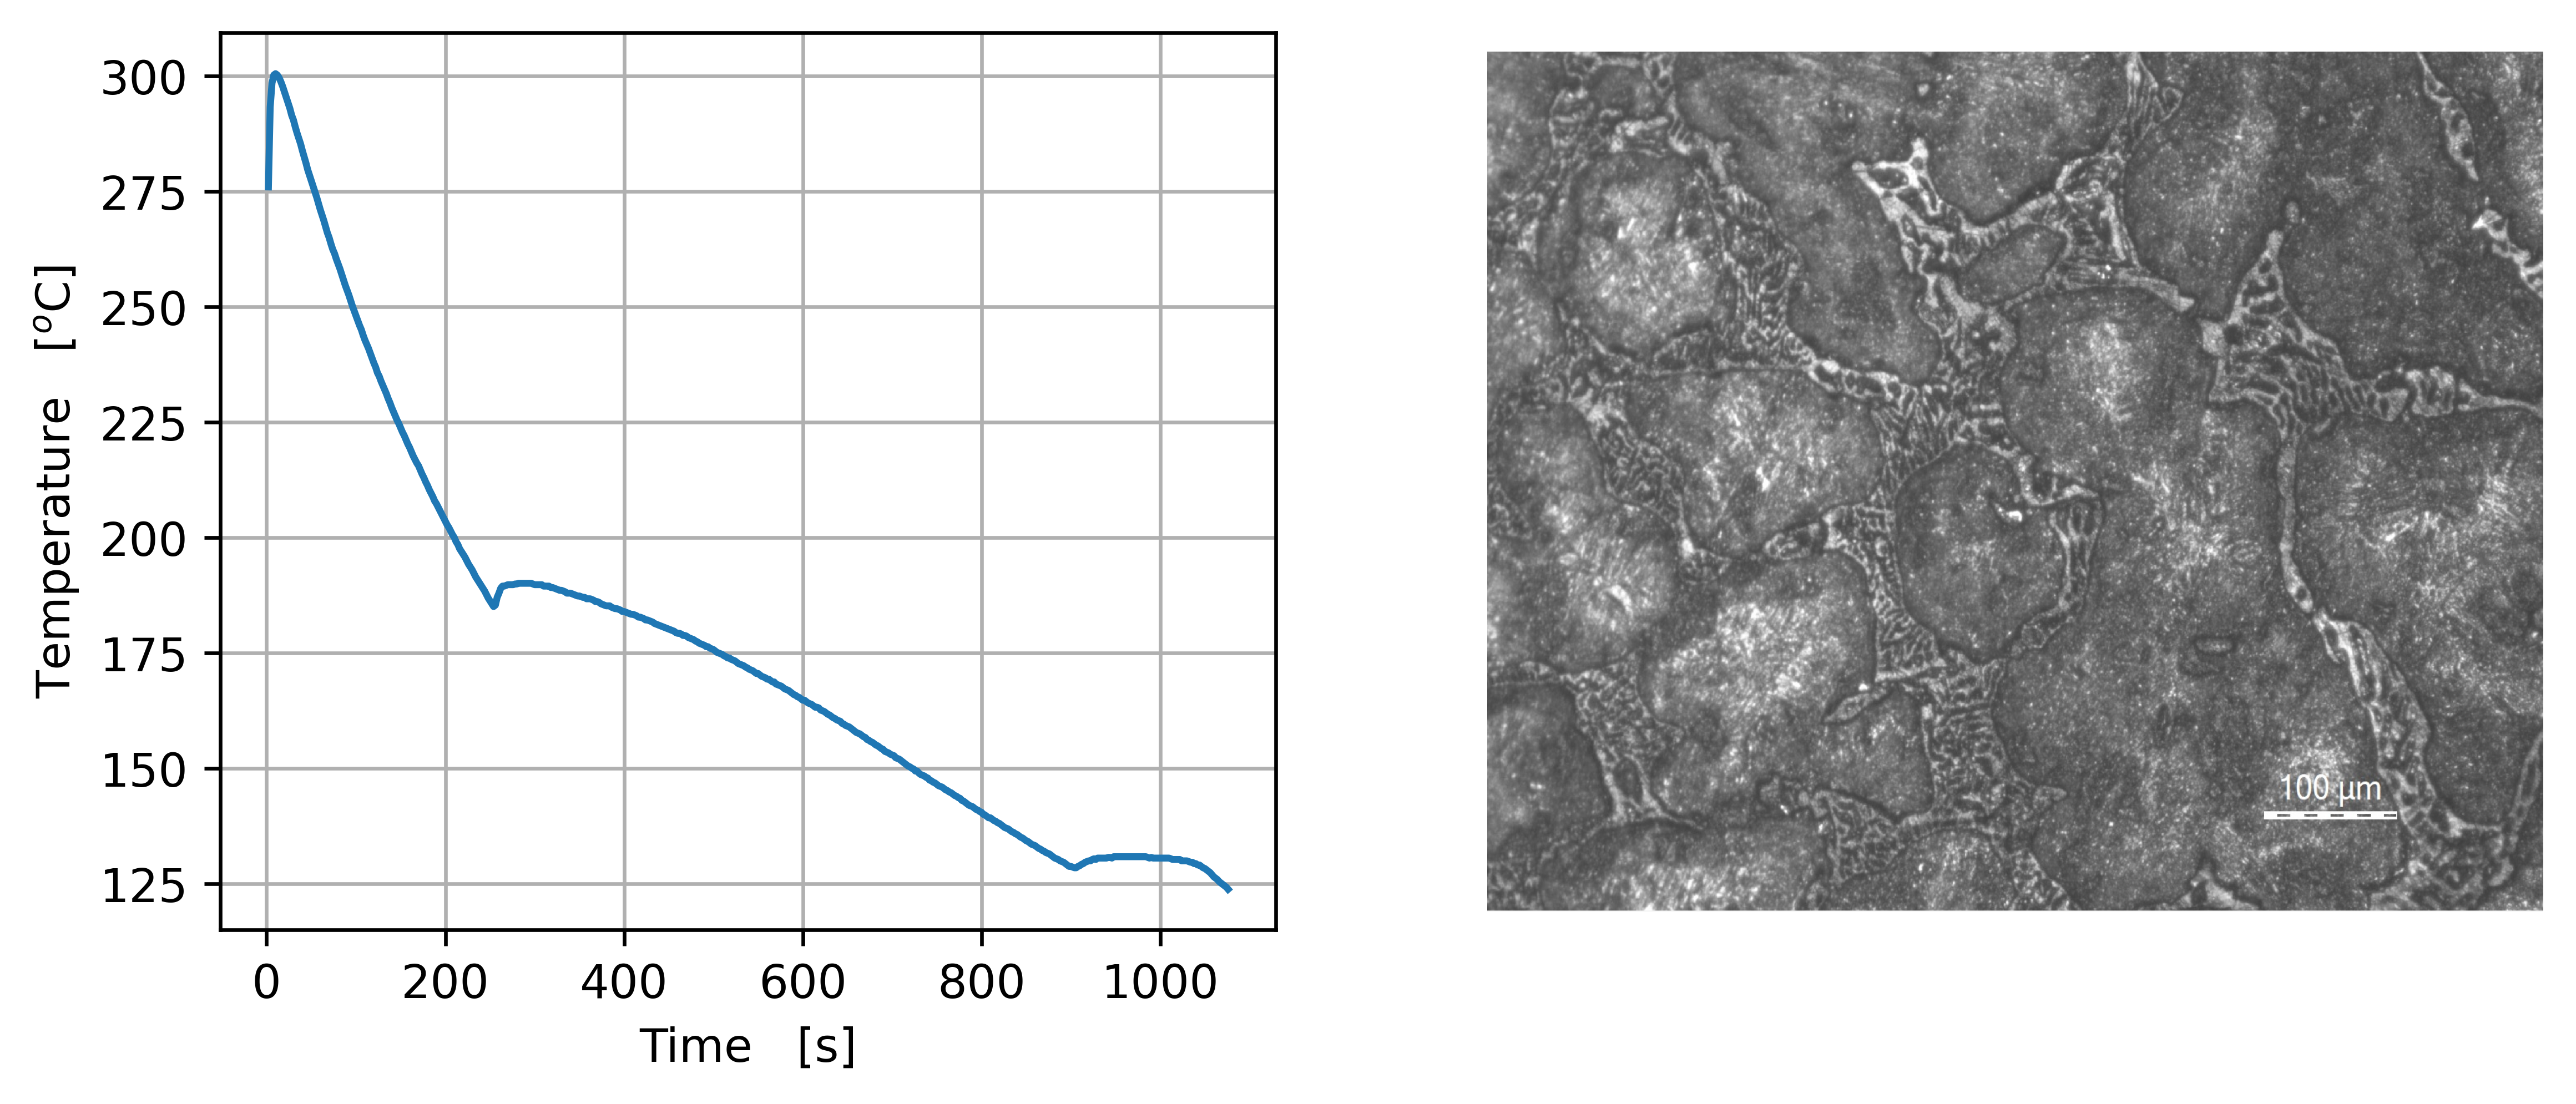
\includegraphics[width=1\linewidth]{plots/q2_25.png}
    \caption{25\% weight-fraction Bismuth cooling curve and micro-structure}
    \label{fig:q2-25}
\end{figure}

\newpage

\begin{figure}[!h!]
    \centering
    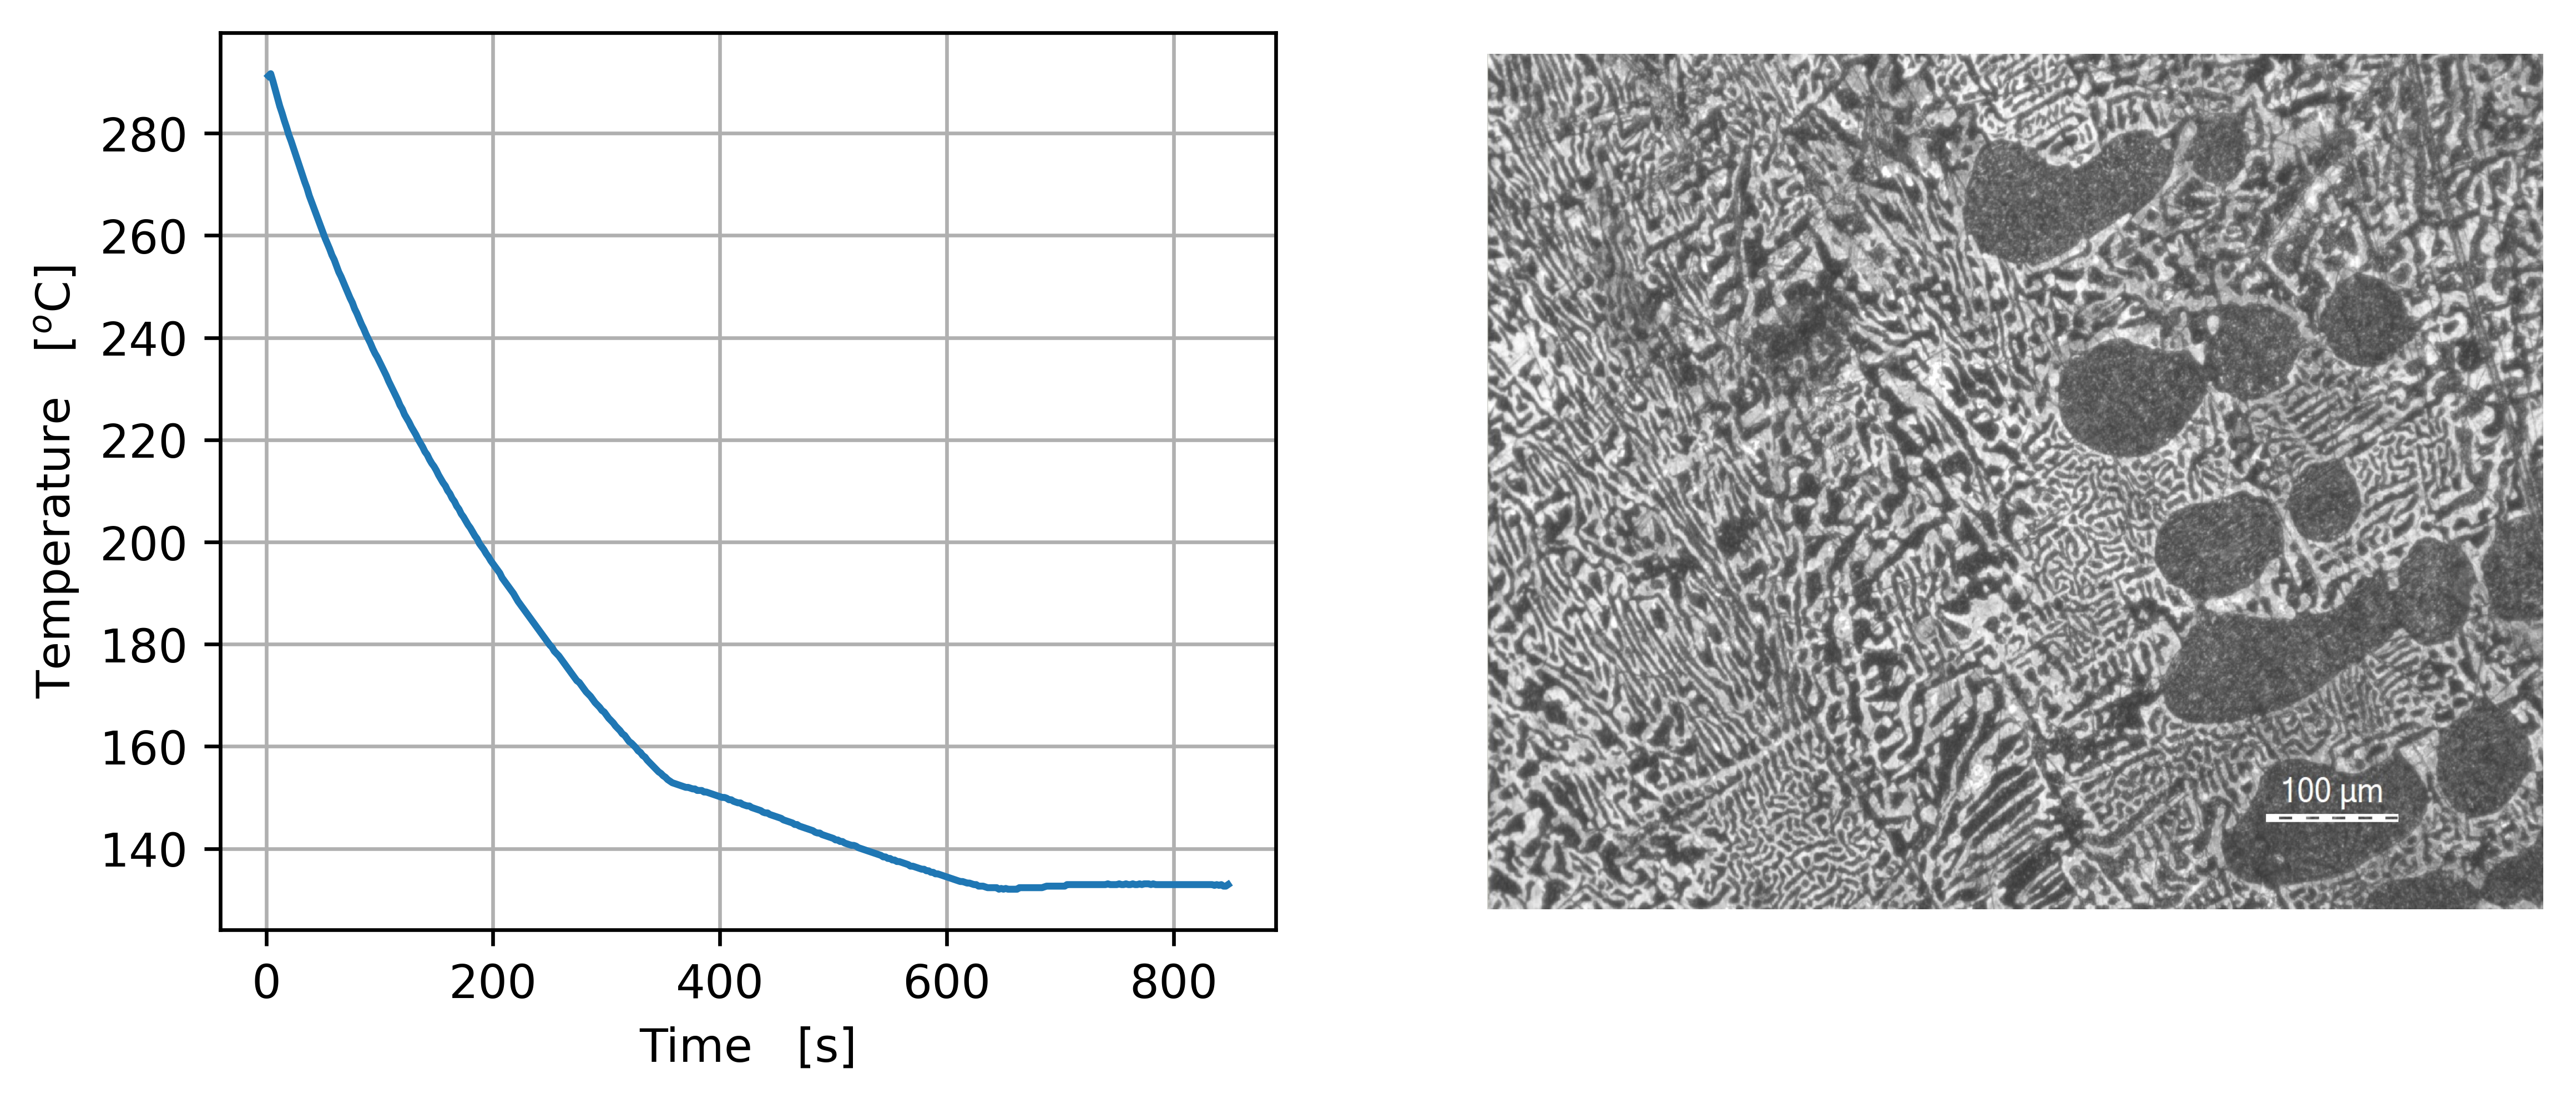
\includegraphics[width=1\linewidth]{plots/q2_50.png}
    \caption{50\% weight-fraction Bismuth cooling curve and micro-structure}
    \label{fig:q2-50}
\end{figure}

\begin{figure}[!h!]
    \centering
    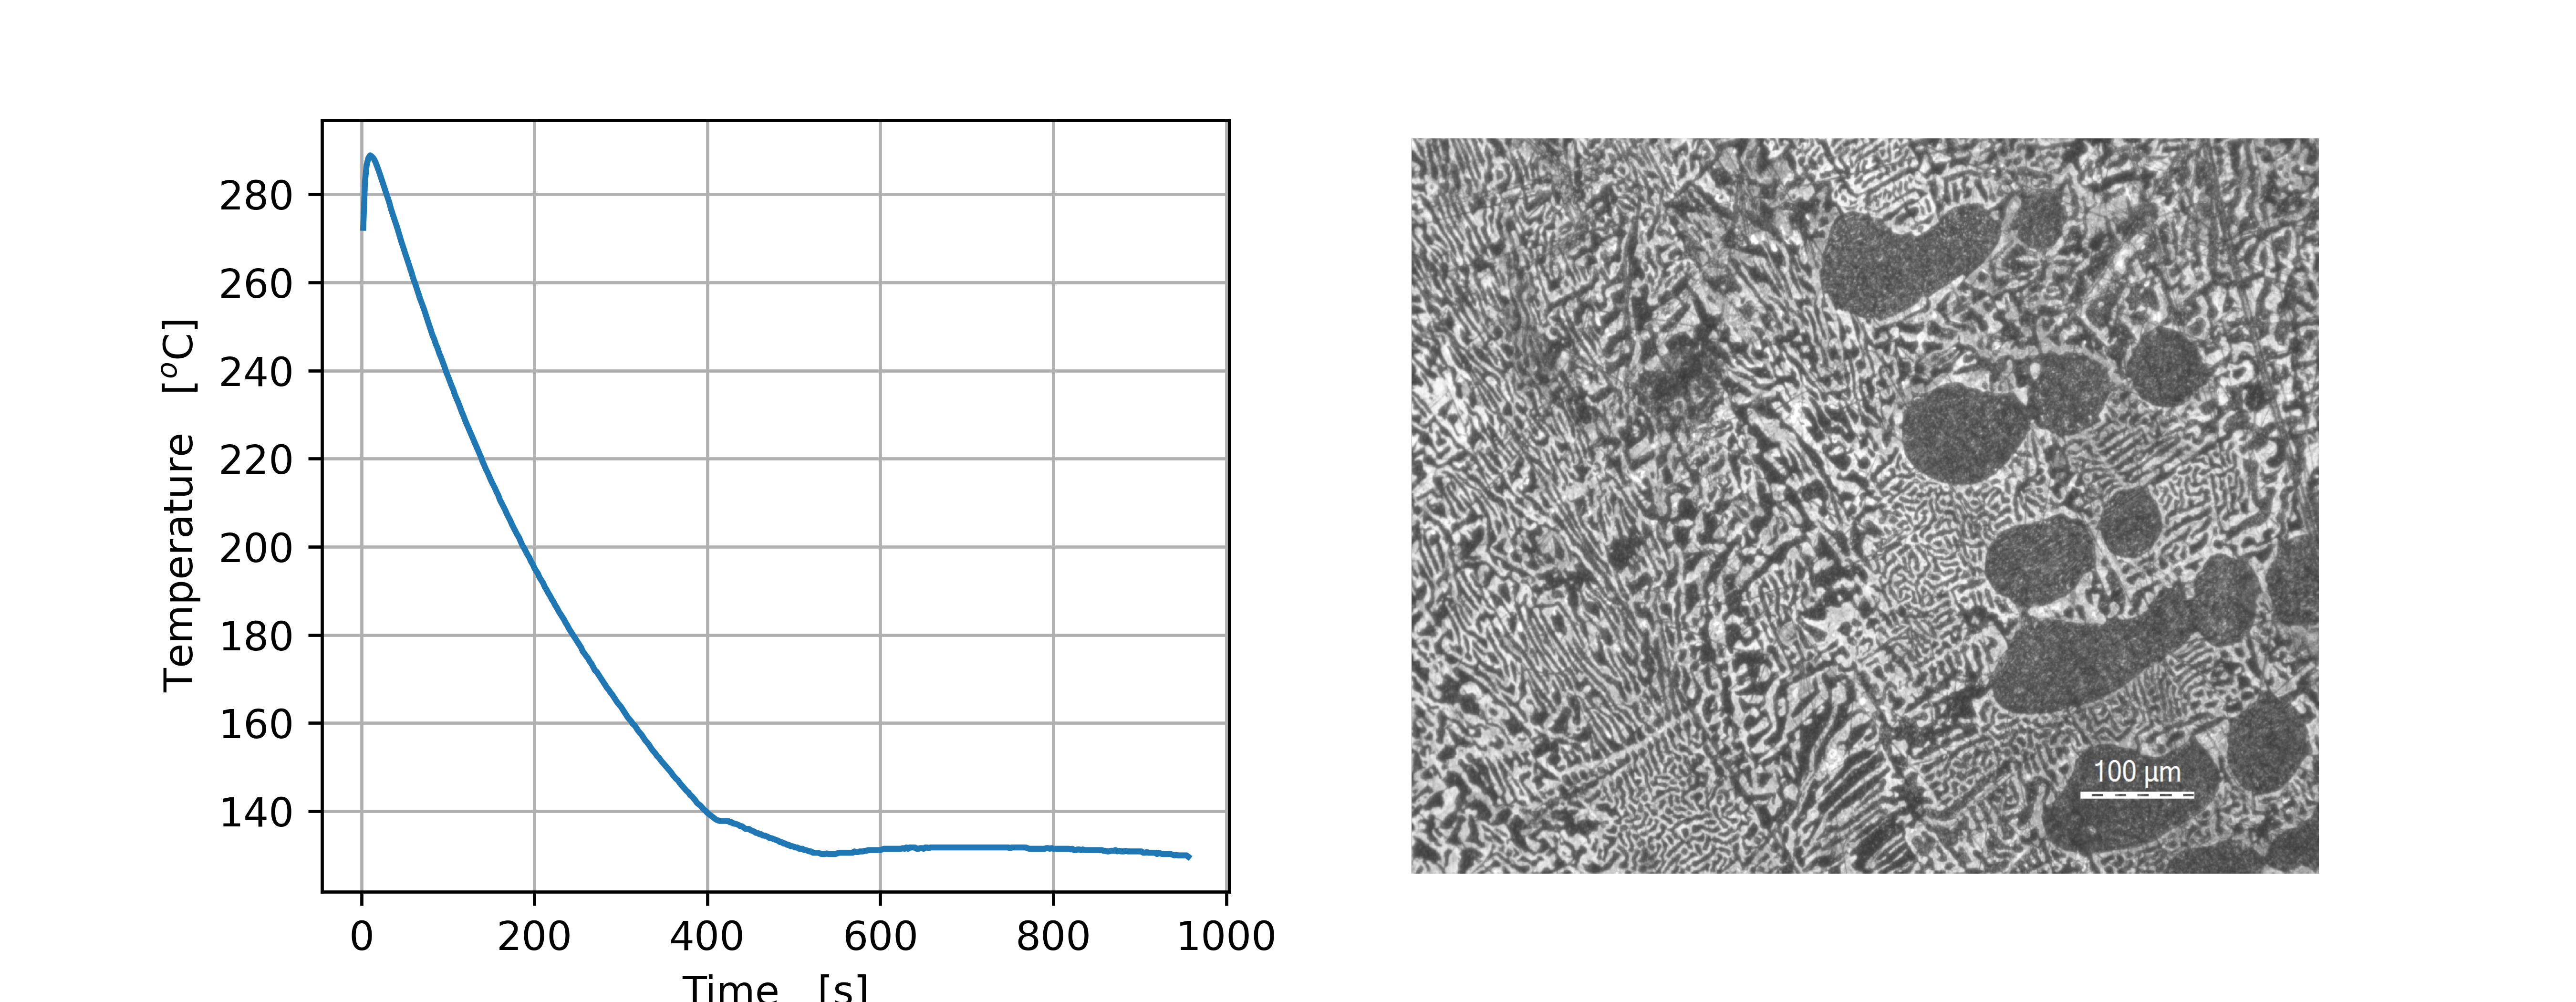
\includegraphics[width=1\linewidth]{plots/q2_55.png}
    \caption{55\% weight-fraction Bismuth cooling curve and micro-structure}
    \label{fig:q2-55}
\end{figure}

\newpage

To continue, we determined the liquidus, solidus, and when applicable the solvus. These values are tabulated below. Notably, the weight-percent of bismuth jumps around outside of a standard 5\% increment. This is simply due to lack of testing for these compositions. 

\begin{table}[!h!]
    \centering
    \def\arraystretch{1.5}
    \caption{Liquidus, Solidus, and Solvus of select samples}
    \begin{tabular}{|c|c|c|c|}
       \toprule
       \hline
        Weight Percent Bismuth & Liquidus & Solvus & Solidus \\ 
         \midrule 
         \hline 
        
        0.0 & 130.0 & -- & --\\ 
          
         \hline 
        
        15.0 & 228.0 & 136.0 & 121.0\\ 
          
         \hline 
        
        25.0 & 190.0 & 130.0 & --\\ 
          
         \hline 
        
        40.0 & 165.0 & 133.0 & --\\ 
          
         \hline 
        
        50.0 & 152.0 & 133.0 & --\\ 
          
         \hline 
        
        55.0 & 138.0 & 131.0 & --\\ 
          
         \hline 
        
        65.0 & 143.0 & 134.0 & --\\ 
          
         \hline 
        
        90.0 & 232.0 & 136.0 & --\\ 
          
         \hline 
    \end{tabular}
    \label{tab:my_label}
\end{table}

Proximally, these are plotted into a scatter plot, super-imposed unto a phase-diagram from the literature \cite{nist}.

\begin{figure}[!h!]
    \centering
    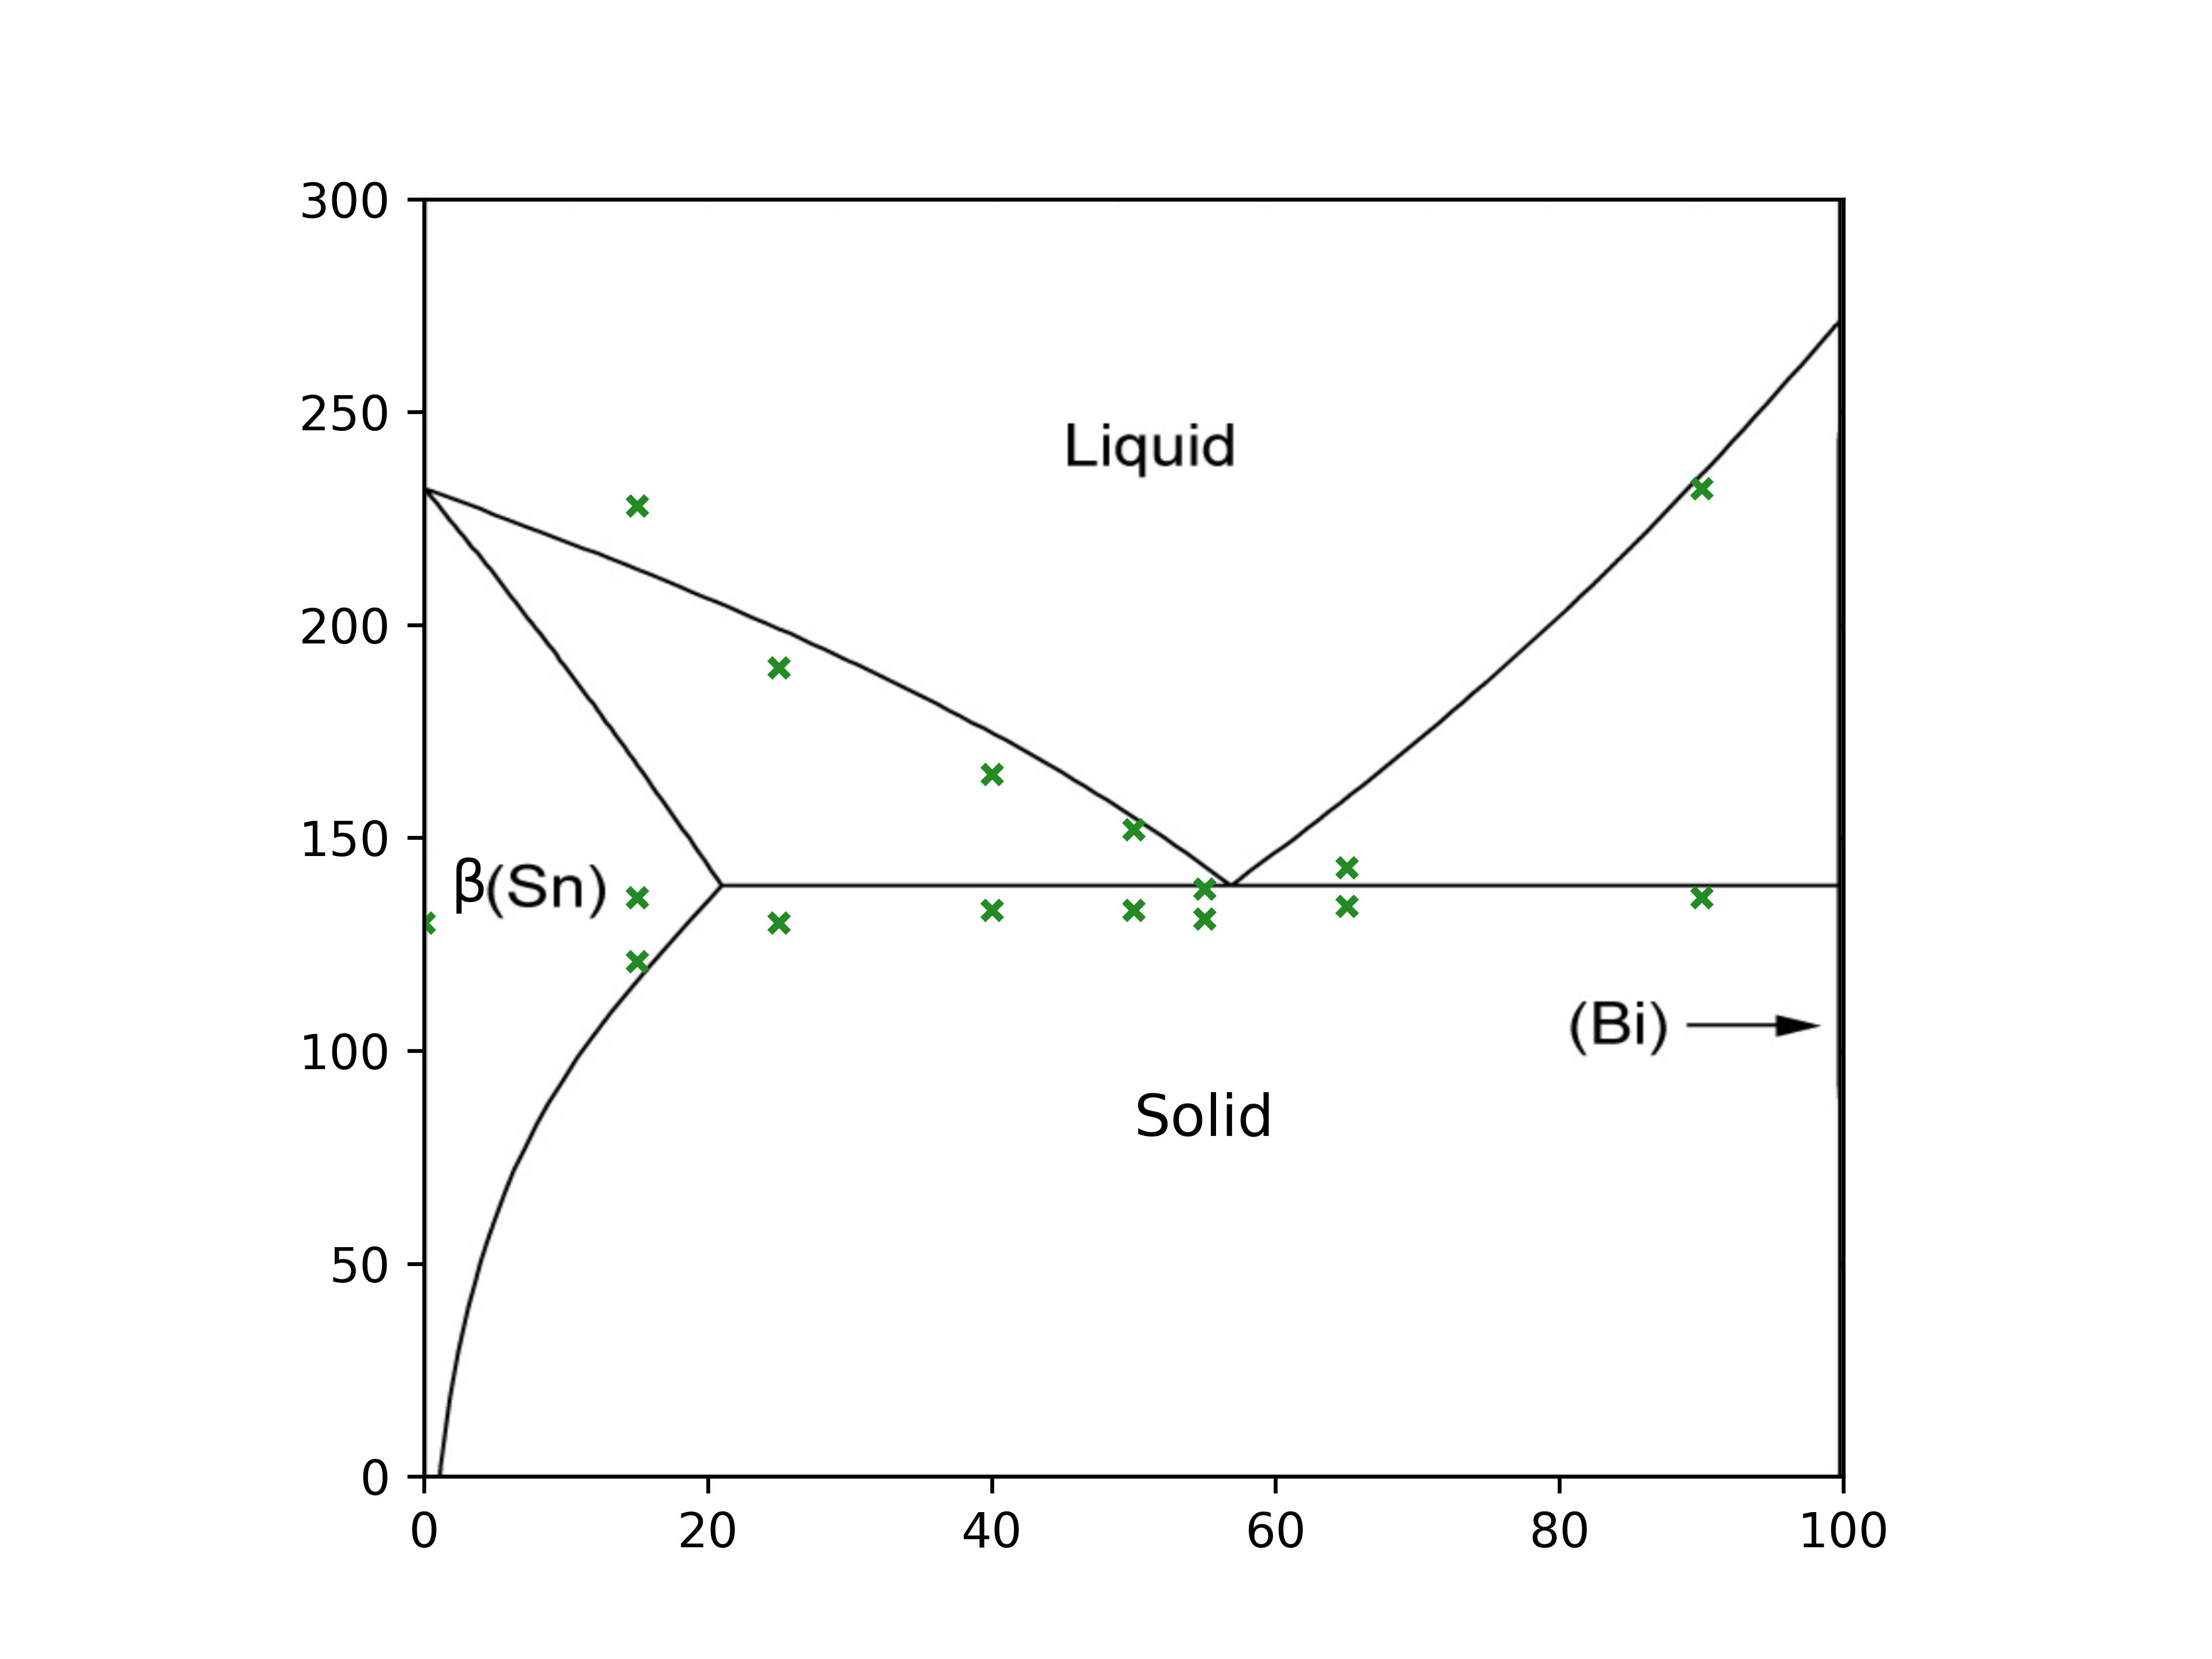
\includegraphics[width=0.5\linewidth]{plots/q4_phase.png}
    \caption{Experimental / Theoretical Phase-Diagram of Sn-Bi system}
    \label{fig:q4fig}
\end{figure}


\newpage
\section{Analysis and Discussion of Results}

We experienced various sources of error pertinent to our data collection regimes undertaken in our experiments. To begin, we had various difficulties with the thermocouple. The first of which was repeatedly clanging the thermocouple against side of the crucible during measurement, yielding incorrect data points. This was particularly evident in our pure metal specimen. Further, we are unsure about the efficacy of the composition labeled on our specimens. This uncertainty propagates, yielding factually incorrect results when compared with literature and expectations. Finally, the methodology employed in determining the liquidus / solidus / solvus points were less than rigorous. We were not utilizing any form of string criteria in our analysis, but rather 'eye-balling' via cursors on the in-lab desktop. All of these sources of error ultimately motivated our decision to utilize ME 330 Section 5's dataset instead of our own.

\newpage
\section{Answers to Questions}

To begin, the liquidus and solidus points are found from determining the inflection points in the cooling curve. The liquidus is the first inflection point, and the solidus the second (in Fig \ref{fig:q1-90}). The pure alloy cooling curve, Fig. \ref{fig:q1-00}, is noticeably different than that of Fig. \ref{fig:q1-90}, in that there is an obvious plateau. This plateau is not due to a lack of energy loss, but rather a transfer of the main mechanism of energy loss from heat transfer to solidification of the metal. In contrast, the alloy cooling curve is not a plateau, but does decrease in rate of heat loss. This is because only some of the energy being lost from the system is in the form of solidification, where some is still liquid and cooling off.

Next, Figs. \ref{fig:q2-00} through \ref{fig:q2-55}. First, the pure tin micro structure yields from large granules of tin forming during cool down. These granules form via solidification propagation normal to the planes of heat transfer. Conversely, in the 25 and 50\% Bismuth samples, bismuth solids formed prior to tin solids. The bismuth solidified in clumps, then forming the grains seen, whereas the tin solidified again via solidification propagation normal to the planes of heat transfer. Finally, the 55\% Bismuth sample is exceedingly close to the eutectic point. Thus, the solid actually forms all at the same time, but still in microscopic clumps.

Next, melting point of tin, as we did not do a reliable full trial of  pure bismuth, was much lower than expected. Because this is not our data, but rather ME 330 Section 5's data, we have no understanding of the problems present in their trials. We assume there was a translational error when logging the data results, and this was actually the solidus line of another cooling curve. Other than this value, we notice that our experimental liquidus and solidus lines match up very closely to the theoretical phase diagram. 

Proximally, again we see that our experimental data matches well with the theoretical phase diagram ---- with some variation. We attribute this variation to three causes. The first is the thermocouple was utilized repeatedly without proper cleaning between each trial. This leads to non-negligible thermal resistance to the thermocouple, causing lower measured temperatures. Further, we can assume the thermocouple is inaccurate as it is a shared item across numerous classes, but we have no way to determine the effects of this. Finally, we were not responsible for constructing the alloys, however we do know how they were formulated. They were formulated utilizing a relatively inaccurate scale, and potentially incorrect 'pure' solutions. Finally, our data allows us to estimate a somewhat close estimate to the eutectic point, albeit lower than true. 

Next, the worksheets are visible in the appendix, Section \ref{appendix}. Perspicuously, the addition of Ti and Cu to Aluminum yields in a higher dislocation density. This is due to the increased amount of grain boundaries between the various phases of the mixture. Of the two, Ti is much more effective at increasing the dislocation density. Increasing the super heat applied to the mold resulted in a lower dislocation density. Conversely, agitating the mold yielded in a higher grain density. 

Finally, we will discuss the formation of columnar and equiaxed grain zones. The conditions which favor columnar growth are higher superheat, slower cooling, lower sub-component weight-fractions, and lack of external agitation. To address the size of the chill zone adjacent to the mold, we can utilize different types of molds, sand has a lower chill zone as it has a much lower thermal conductivity than graphite. Proximally, the 1.5\% Cu in Al in the graphite mold superheated to 50 $^o$C had the most uniform macrostructure. Finally, the benefits of having a uniform macrostructure is the material will have constant material properties throughout and not have any one location significantly more likely than any another to fail. Conversely, a lower uniformaity macrostructure has the advantages of having localized applications. For example, if you want the middle of the material to be very ductile, and the external to be very strong, one uniform material would not suffice ---- but multi-structured materials will. 



\section{Conclusions}
To investigate the phase-diagrams and casting effects on micro structures, we investigated the cooling curve of the Bi-Sn system, and investigated the macro-structures of various Aluminum mixtures dependant on material composition, casting temperature, and casting mold type. We determined the cooling curve of various compositions of the Bi-Sn system and, from these curves, extracted the liquidus, solidus, and solvus points, when applicable. We found our experimentally determine inflection points to be a near fit to the theoretical phase-diagram found from \cite{nist}. Further, we determined that sand cast mold specimens cooled much slower, and more uniformly, causing a hole to form at the center of the specimen; whereas graphite cast mold specimens had a divot form at the top ---- where the air was the main coolant ---- as the top cooled much slower than the sides and bottom. Further, we determined that Titanium had the most impact per weight-percent added to the system on the system's grain structure. Finally, we determined that a decrease in super-heat and a presence of specimen agitation during cooling led to more columnar and large granules. 


\newpage
\section{Appendix A}\label{appendix}

\begin{figure}[!h!]
    \centering
    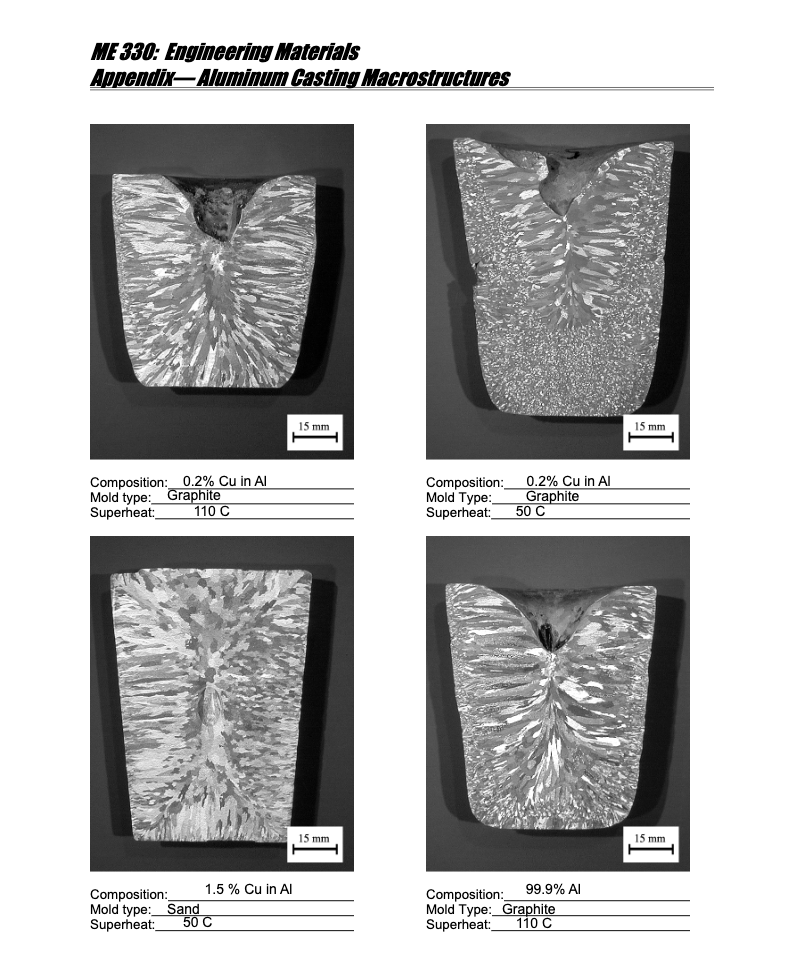
\includegraphics[width=\linewidth]{Lab4/ws_p1.png}
\end{figure}
\newpage
\begin{figure}[!h!]
    \centering
    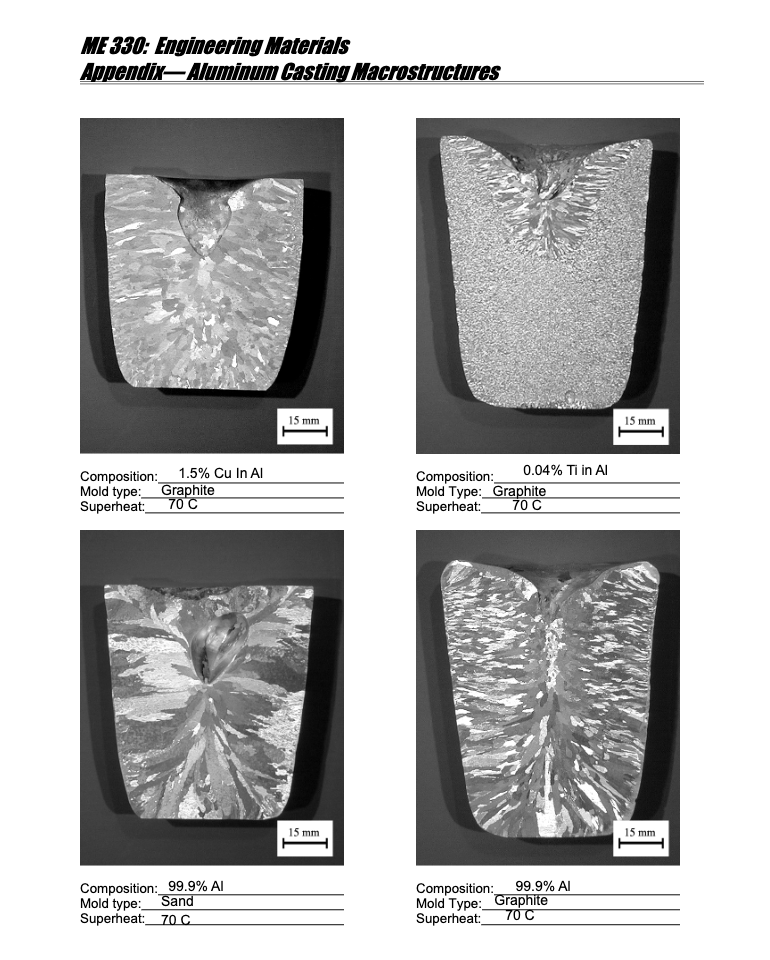
\includegraphics[width=\linewidth]{Lab4/ws_p2.png}
\end{figure}
\newpage
\begin{figure}[!h!]
    \centering
    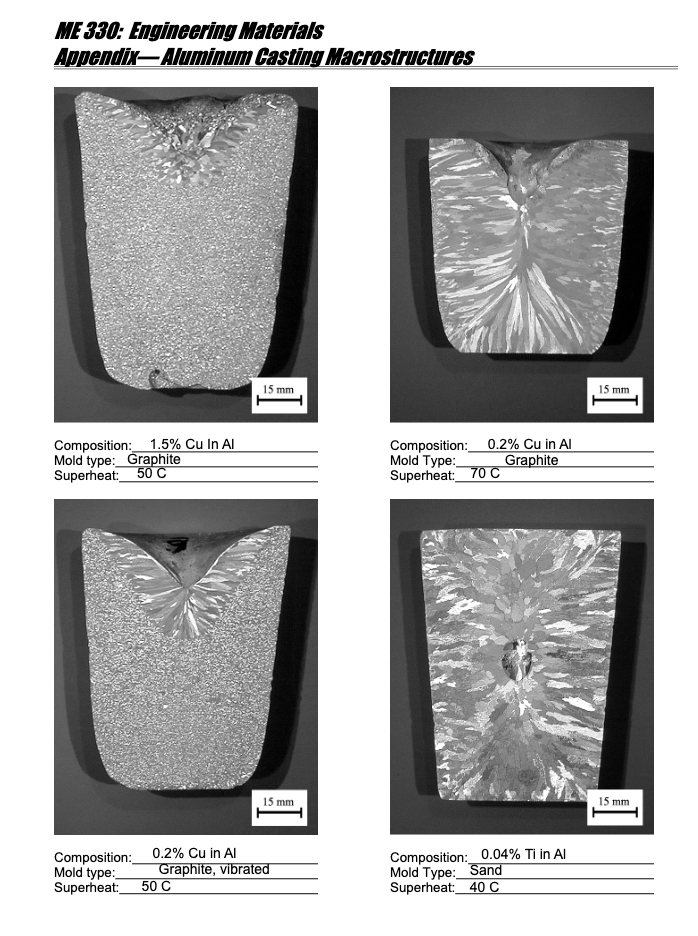
\includegraphics[width=\linewidth]{Lab4/ws_p3.png}
\end{figure}

\section{Bibliography}

\printbibliography[heading=none]

\end{document}